\chapter{Tasks of the project}
\section{Task Identification}
The project is composed of the following tasks:

\begin{table}[H]
	\centering
	\begin{tabular}{ r | l } 
		\textbf{PHASE} & \textbf{TASKS} \\ \hline
		\textbf{RASD} & T1: Requirement Specification \\
					  & T2: UML Diagrams \\
			          & T3: Alloy Model \\ \hline
		\textbf{DD} & T4: Architectural Design \\
					& T5: Algorithm Design \\
					& T6: Requirement Traceability \\ \hline
		\textbf{ITPD} & T7: ITPD \\ \hline
		\textbf{PM} & T8: FP \\
					& T9: COCOMO \\
					& T10: Task Identification \\
					& T11: Resources Allocation \\
					& T12: Risk Management \\ \hline
		\textbf{DEVELOPMENT} & T13: Backend \\
							 & T14: Frontend \\ \hline
		\textbf{TESTING} & T15: Unit Testing \\
						 & T16: Integration Testing
	\end{tabular}
\end{table}

\pagebreak

\section{Phase Deadline}
Here are shown the deadlines of each phase. Please note that there are no fixed deadline for the development phase nor for the testing phase. Therefore the length of the tasks in the Gantt Diagram (\ref{gantt}) are purely symbolic.

\begin{table}[H]
	\centering
	\begin{tabular}{ r | l } 
		\textbf{PHASE} & \textbf{DEADLINE} \\ \hline
		\textbf{RASD} & 06/11/2015 \\
		\textbf{DD} & 04/12/2015 \\
		\textbf{ITPD} & 20/01/2016 \\
		\textbf{PM} & 02/02/2016 \\
		\textbf{DEVELOPMENT} & // \\
		\textbf{TESTING} & // \\
	\end{tabular}
\end{table}

\section{Gantt Diagram}

\begin{figure}[H]
	\centering
	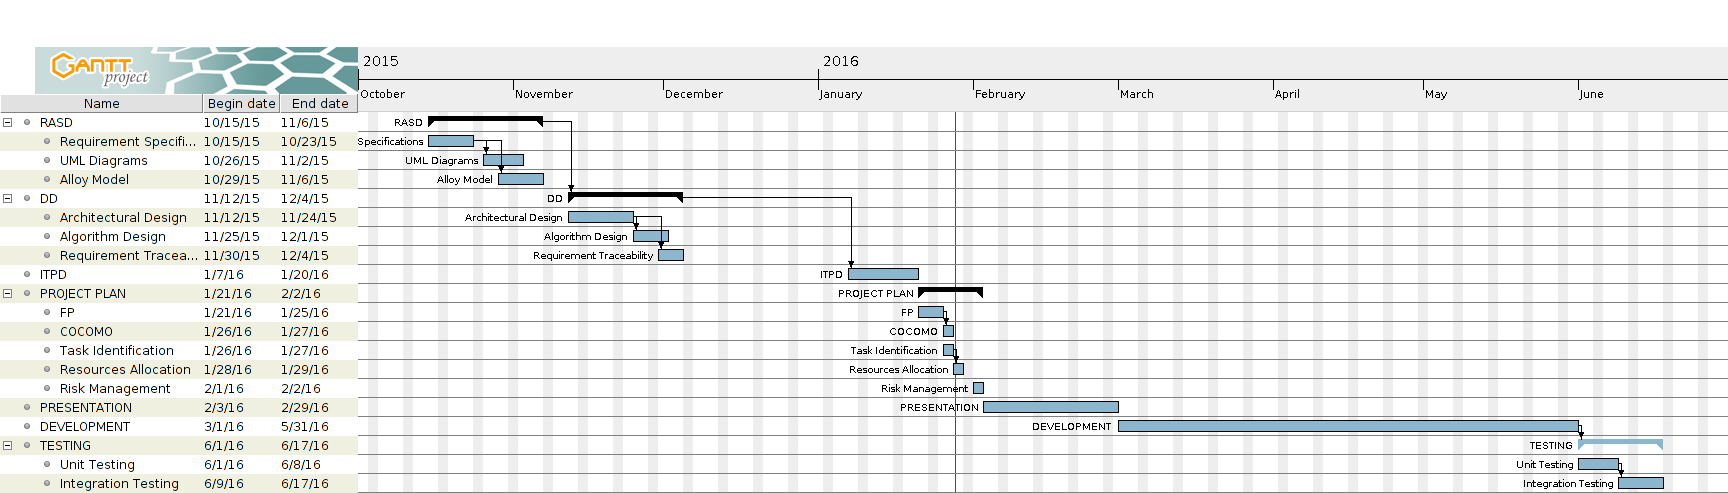
\includegraphics[angle=90,scale=0.4]{Tasks/gantt}
	\label{gantt}
\end{figure}
